\documentclass[11pt]{article}
\usepackage[utf8]{inputenc}
\usepackage[english, ngerman]{babel}
\usepackage{amsmath,amsthm,verbatim,amssymb,amsfonts,amscd}
\usepackage{enumerate}
\usepackage{listings}
\usepackage{courier}
\usepackage[]{graphicx}
\usepackage[]{epstopdf}
\usepackage[margin=1in]{geometry}
\lstset{
  numbers=left,
  language=C,
  basicstyle=\footnotesize\ttfamily,
  breaklines=true,
  morekeywords={function, NIL, new}
}
\newcommand{\abs}[1]{\left| #1 \right| }
\setlength{\parindent}{0pt} 

\author{
  Felix Schrader, 3053850 \\ 
  Jens Duffert, 2843110 \\
  Eduard Sauter, 3053470
}
\title{Datenstrukturen und Algorithmen: Haus\"ubung 6}
\begin{document}
\maketitle
\subsection*{Aufgabe 1}
\begin{enumerate}[a)]
  \item $ $
    \begin{figure}[h!]
      \centering
      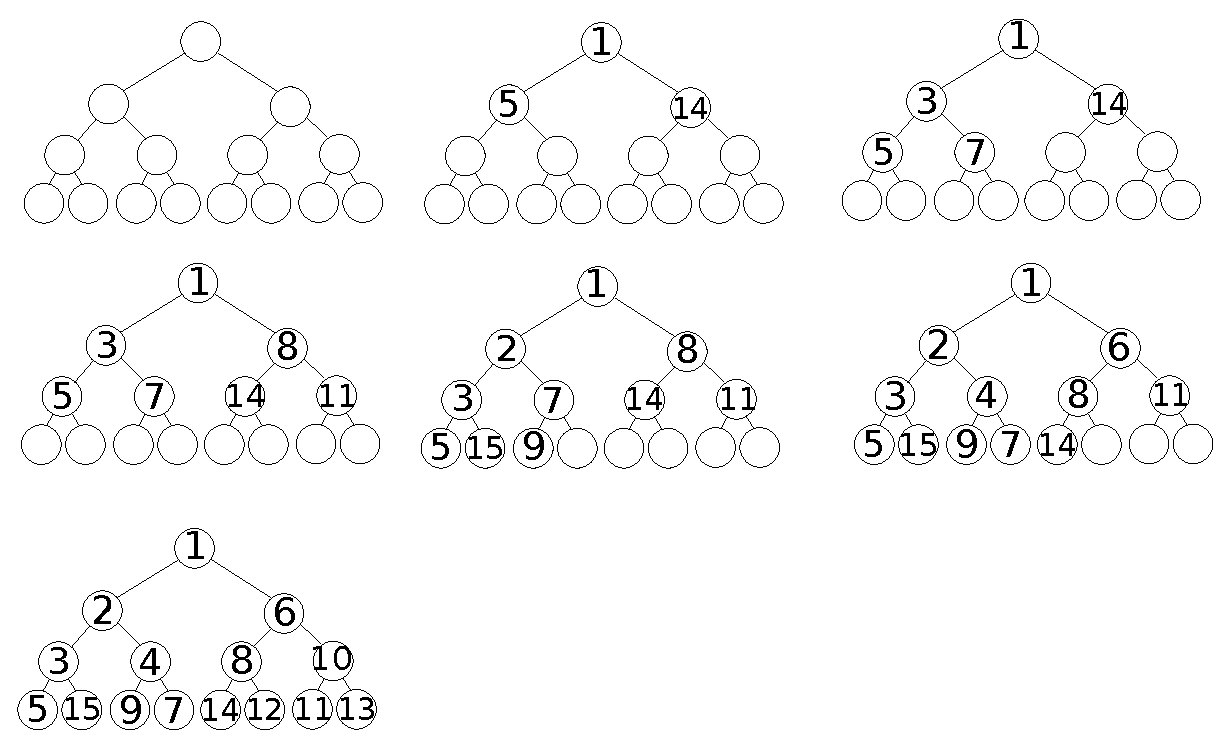
\includegraphics[width=\textwidth]{a1a_trees}
      \caption{Zwischenschritte der Konstruktion des Heaps aus dem gegebenen Schlüssel}
    \end{figure}
  \item $ $
    \begin{figure}[h!]
      \centering
      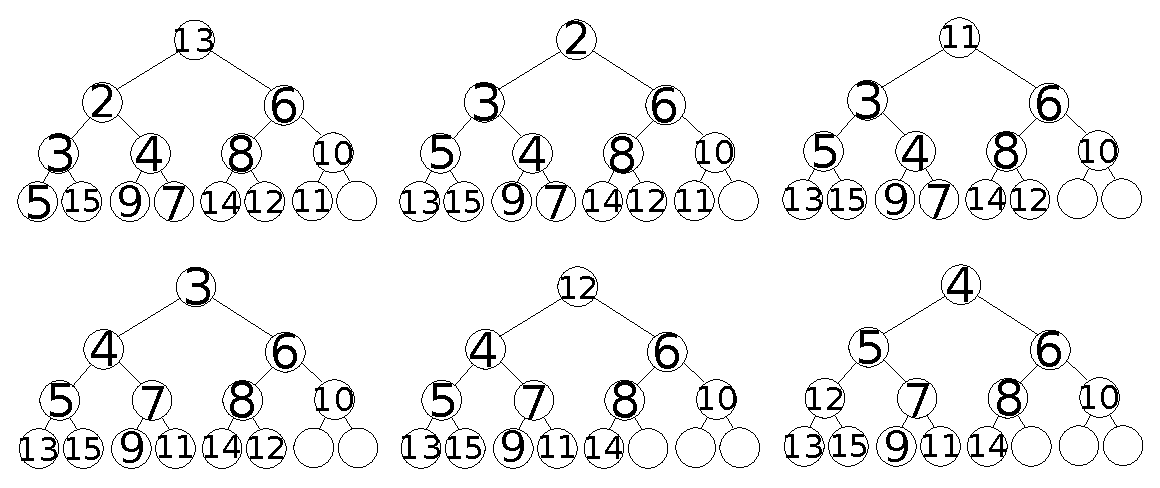
\includegraphics[width=\textwidth]{a1b_trees}
      \caption{Heap nach Entfernen der Wurzel und Sortieren}
    \end{figure}
    \pagebreak
  \item $ $
    \begin{figure}[h!]
      \centering
      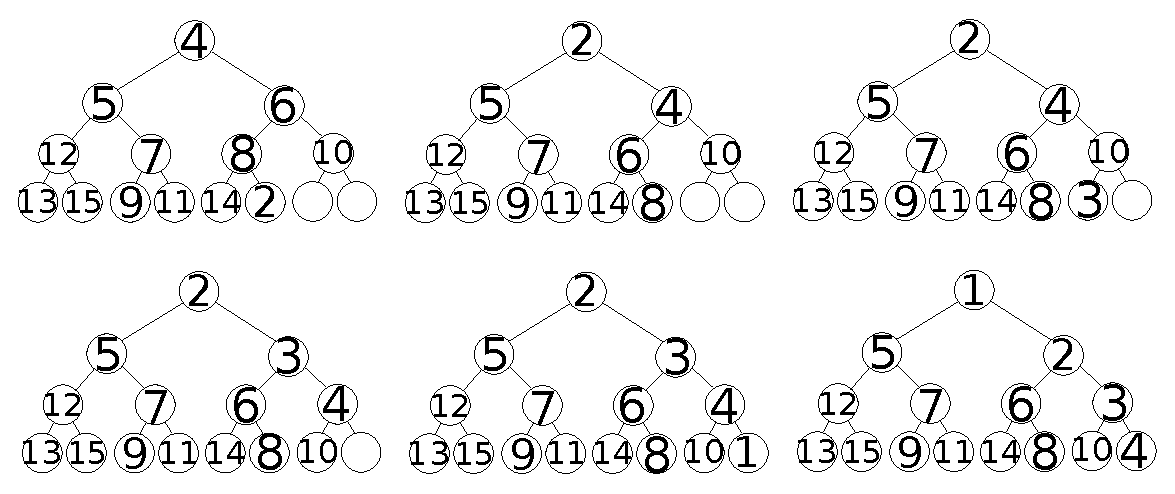
\includegraphics[width=\textwidth]{a1c_trees}
      \caption{Heap nach Hinzufügen von 2, 3, 1 und Sortieren}
    \end{figure}
\end{enumerate}
\newpage
\subsection*{Aufgabe 2}
\lstinputlisting{knapsack.js}

\begin{description}
  \item[Laufzeiten der ADT Queues] $ $
    \begin{table}[h!]
      \centering
      \begin{tabular}{c c c c c c}
                             & Array Unsortiert & Array Sortiert   & Heap \\
          \texttt{insert(x)} & $\mathcal{O}(1)$ & $\mathcal{O}(n)$ & $\mathcal{O}(\log n)$ \\
          \texttt{delMax(x)} & $\mathcal{O}(n)$ & $\mathcal{O}(1)$ & $\mathcal{O}(\log n)$ \\
          \texttt{delMin(x)} & $\mathcal{O}(n)$ & $\mathcal{O}(1)$ & $\mathcal{O}(\log n)$ \\
         \end{tabular}
    \end{table}

  \item[Worst-Case Laufzeiten]
    Es sein $n = \texttt{len(items)}$.
    Im schlimmsten Fall passen alle Elemente in den Rucksack 
    (Ist das Wirklich so schlimm?). Zeile 4 wird in jedem Fall $n$ mal
    ausgeführt. Im Worst-Case werden auch Zeilen 11 bis 13 $n$ mal 
    ausgeführt. Es folgt also für die Laufzeiten von \texttt{KnapsackGreedy()}
    \begin{table}[h!]
      \centering
      \begin{tabular}{c c c c c c}
                             Array Unsortiert & Array Sortiert   & Heap \\
          
        $\mathcal{O}(n^2)$ & $\mathcal{O}(n^2)$ & $\mathcal{O}(n \log n)$ \\
      \end{tabular}
    \end{table}
    

  
\end{description}



  

\end{document}
